%% Appendix
\appendix

\section{Additional NS Examples}
\label{appendix:MoreNsExamples}


\subsection{Motivating Examples --- Explanation}


Observe the simple program depicted in Listing~\ref{lst:MotivatingExample1Ser}. Each  {\color{ForestGreen}$\blacklozenge_\text{main}$} gives rise to a fresh in-flight request. The variable ``X'' is global, and shared among all in-flight requests, while the variable ``y'' is local variable, per each request. 
%
As there are no yields, it is straightforward to see that the program is trivially serializable, with every request {\color{ForestGreen}$\blacklozenge_\text{main}$}: (i) assigning 1 to the global variable X; (ii) assigning to y to have the value of X, i.e., always 1; (iii) assigning to X the value 0; and (iv) returning the response y ({\color{red}$\blacklozenge_1$}). This results to every (request,response) pair to be of the form {\color{ForestGreen}$\blacklozenge_\text{main}$}/{\color{red}$\blacklozenge_1$}.
%
The program is slightly altered (in Listing~\ref{lst:MotivatingExample2NonSer}), by adding a yield operation between the aforementioned steps (i) and (ii). Now, by running two {\color{ForestGreen}$\blacklozenge_\text{main}$} requests that interleave, it is possible to attain a {\color{ForestGreen}$\blacklozenge_\text{main}$}/{\color{red}$\blacklozenge_0$} request/response pair, which is unattainable in any serial execution of Listing~\ref{lst:MotivatingExample2NonSer} --- as any such serial execution is equivalent to Listing~\ref{lst:MotivatingExample1Ser}, which always responds {\color{red}$\blacklozenge_1$} to any request {\color{ForestGreen}$\blacklozenge_\text{main}$}.


The program is altered once again in in Listing~\ref{lst:MotivatingExample3Ser}, by adding a fresh global variable ``L'', indicating if the critical section is locked ($L=1$) or not ($L=0$).
By adding a global lock variable, even if an interleaving occurs after yielding, the lock will allow only the first request to terminate, and will then release the lock for the next request. Hence, despite having yields, we attain serializable executions, and only {\color{ForestGreen}$\blacklozenge_\text{main}$}/{\color{red}$\blacklozenge_1$} request/response pairs are produced, similar to the original program in Listing~\ref{lst:MotivatingExample1Ser}.
%
This simple example demonstrates the motivation for automatic serializability checking, as even small, toy programs can be surprisingly difficult to reason about when assessing their serializable behavior.



\subsection{Motivating Examples \#1}
\label{appendix:subsec::Ex1A:NS}


For our third motivating example, presented in Listing~\ref{lst:MotivatingExample1Ser}, we have the following NS:


%\begin{minipage}[t]{0.3\textwidth}
%	\begin{lstlisting}[caption={Without yield or lock (serializable)}]
%	request main: 
%		X := 1 
%		// no yield
%		y := X 
%		X := 0
%		return y 
%	\end{lstlisting}
%\end{minipage}

\begin{figure}[!htbp]
	\centering
	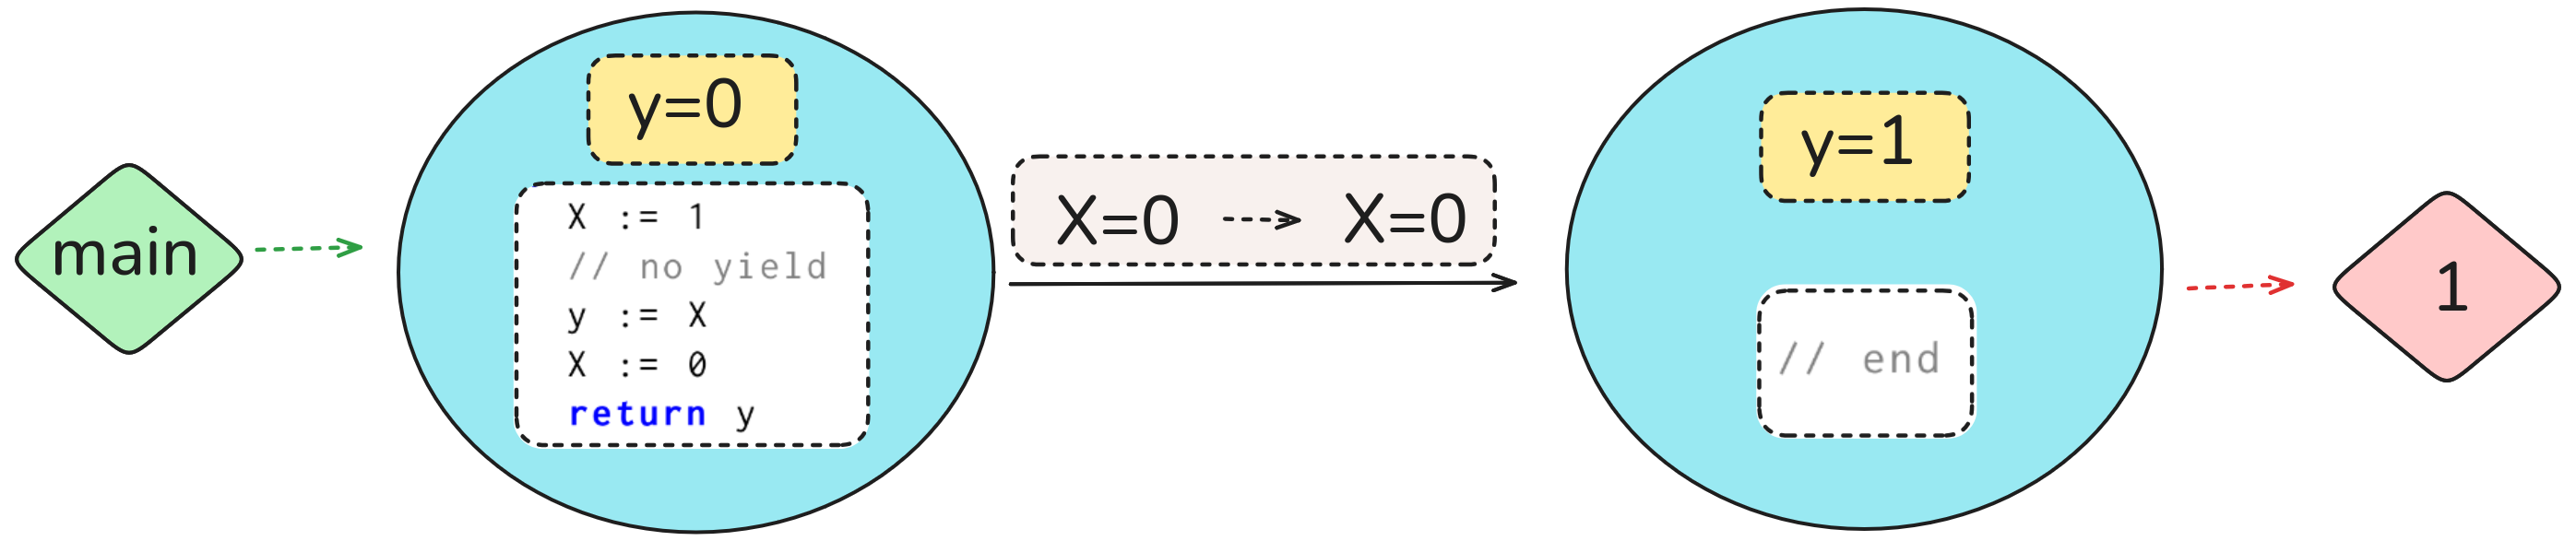
\includegraphics[width=0.9\textwidth]{plots/code_1_NS.png}
	\caption{Network System for interleaving executions of Listing~\ref{lst:MotivatingExample1Ser} program.}
	\label{fig:code1ExampleNS}
\end{figure}


\begin{figure}[!htbp]
	\centering
	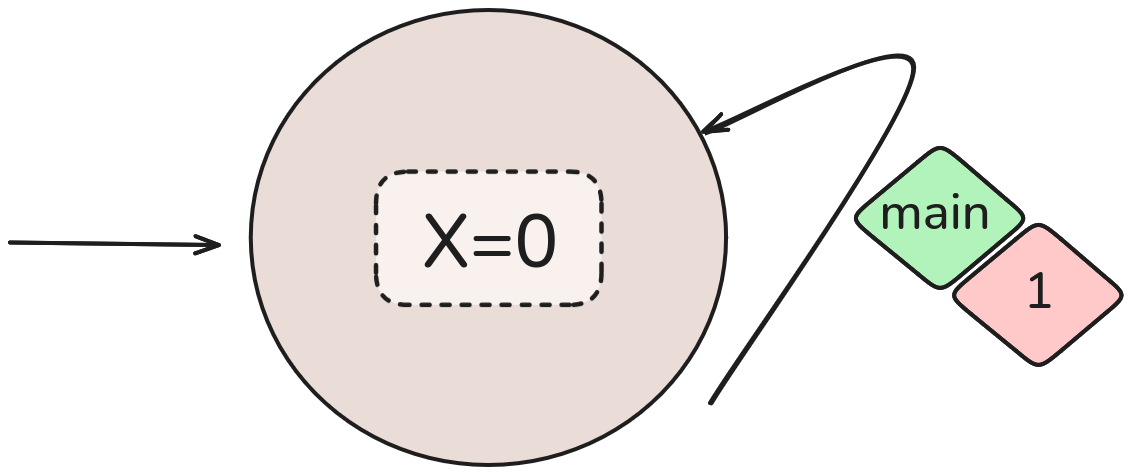
\includegraphics[width=0.35\textwidth]{plots/code_1_NFA.png}
	\caption{NFA for serialized executions of Listing~\ref{lst:MotivatingExample1Ser} program.}
	\label{fig:code1ExampleNFA}
\end{figure}



\begin{figure}[!htbp]
	\centering
	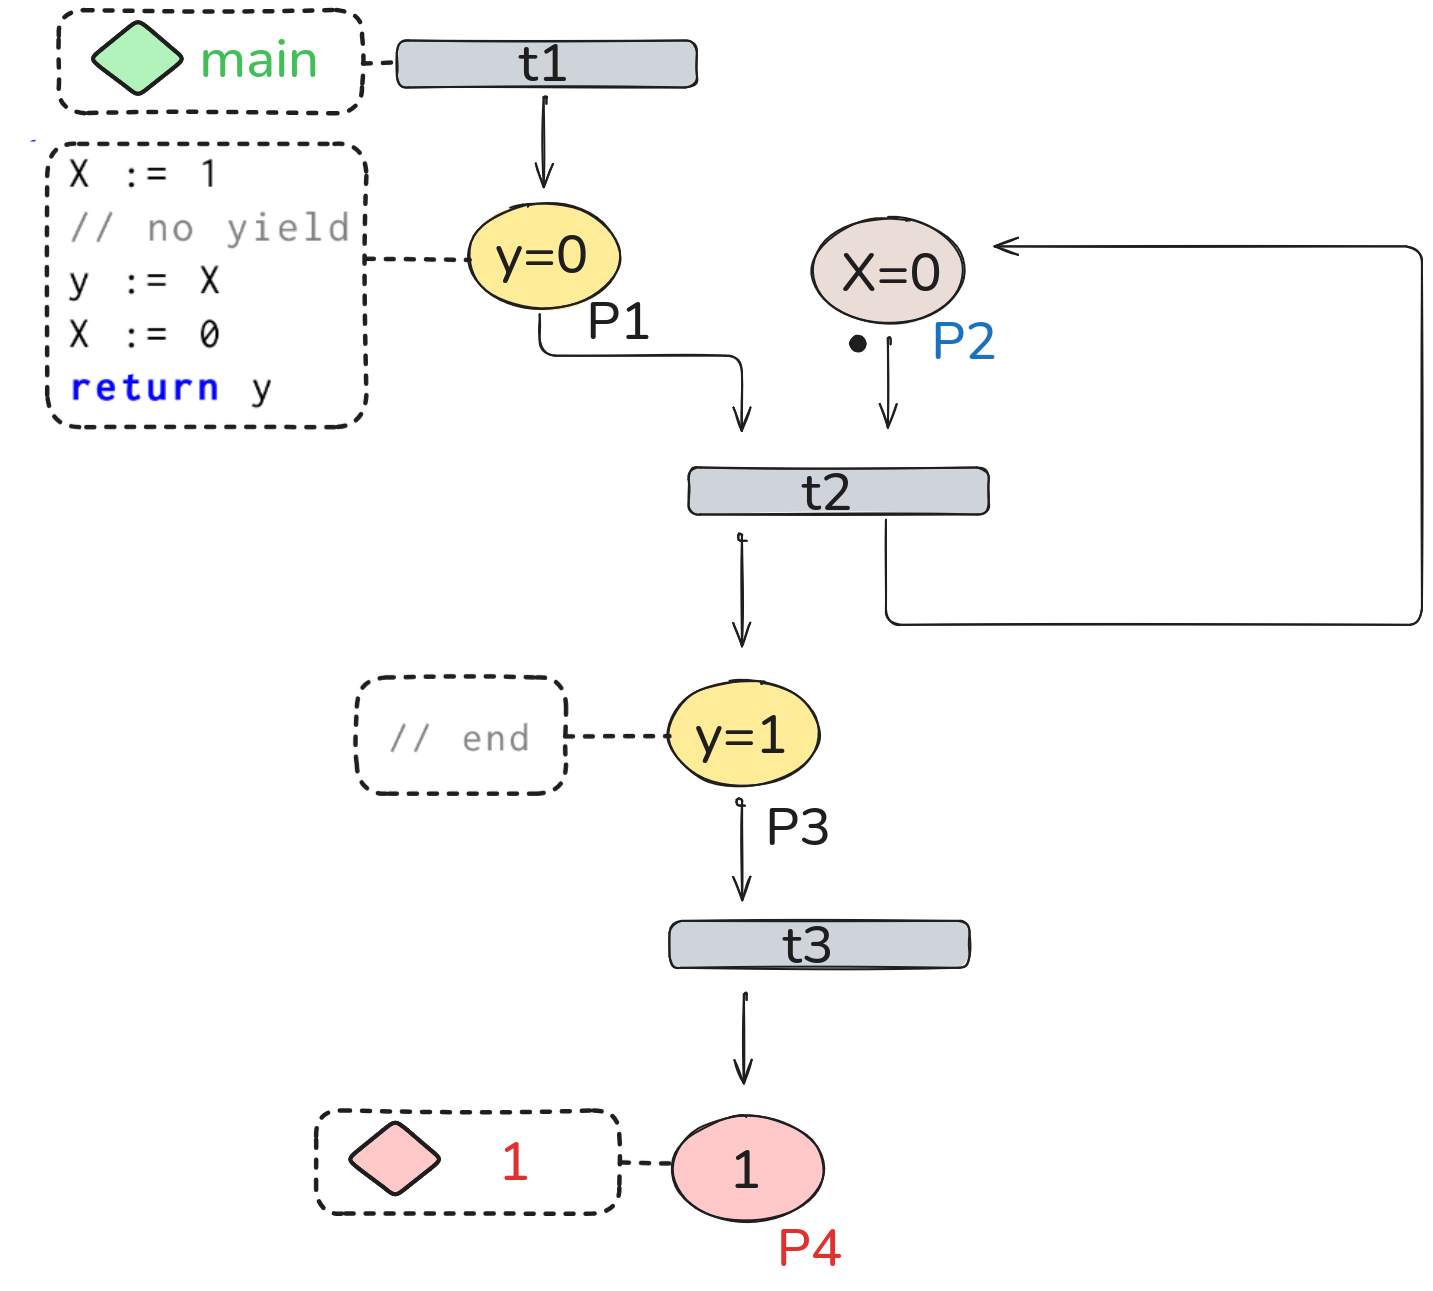
\includegraphics[width=0.6\textwidth]{plots/code_1_PN_with_annotation.png}
	\caption{Petri Net for interleaving executions of Listing~\ref{lst:MotivatingExample1Ser} program.}
	\label{fig:code1ExamplePN}
\end{figure}

%

\subsection{Motivating Examples \#2}
\label{appendix:subsec::Ex1B:NS}

For details, see the main text (Sec.~\ref{sec:problem-definition}).


\subsection{Motivating Examples \#3}
\label{appendix:subsec:Ex1C:NS}

For our third motivating example, presented in Listing~\ref{lst:MotivatingExample3Ser}, we have the following NS:

%\begin{minipage}[t]{0.3\textwidth}
%	\begin{lstlisting}[caption={With yield and lock (serializable)}]
%		request foo: 
%			// lock
%			while (L == 1): 
%				yield
%			L := 1 
%		
%			X := 1
%			yield
%			y := X 
%			X := 0
%		
%			// unlock    
%			L := 0
%			return y 
%	\end{lstlisting}
%\end{minipage}
%
%This program corresponds to the following Network System (NS):

\begin{figure}[!htbp]
	\centering
	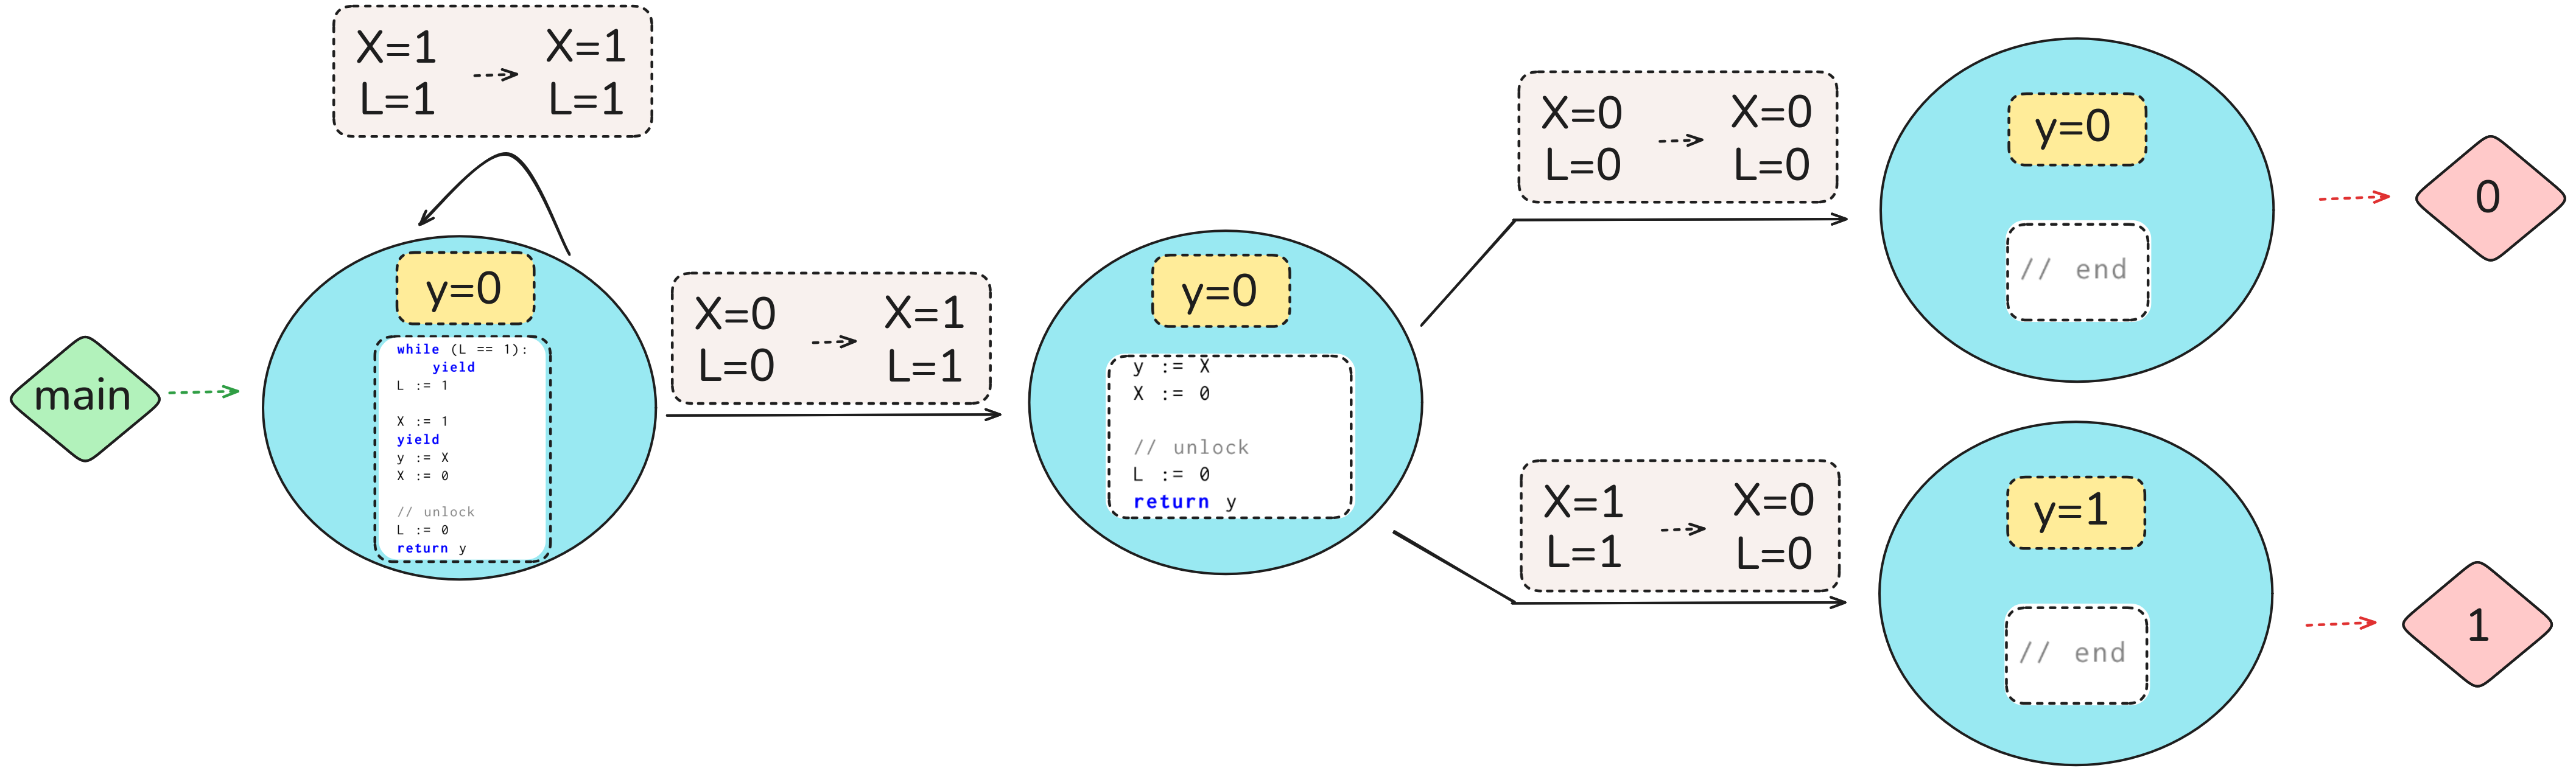
\includegraphics[width=1.1\textwidth]{plots/code_3_NS.png}
	\caption{Network System for interleaving executions of Listing~\ref{lst:MotivatingExample3Ser} program.}
	\label{fig:code3ExampleNS}
\end{figure}


\begin{figure}[!htbp]
	\centering
	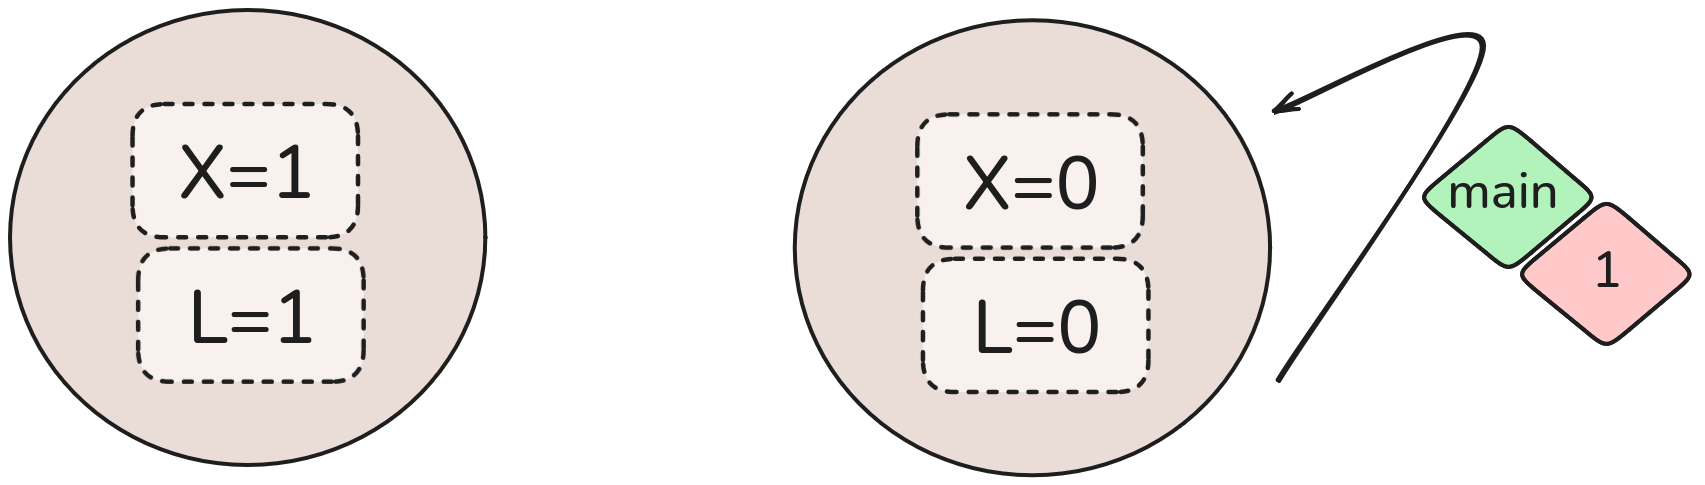
\includegraphics[width=0.4\textwidth]{plots/code_3_NFA.png}
	\caption{NFA for serialized executions of Listing~\ref{lst:MotivatingExample3Ser} program.}
	\label{fig:code3ExampleNFA}
\end{figure}



\begin{figure}[!htbp]
	\centering
	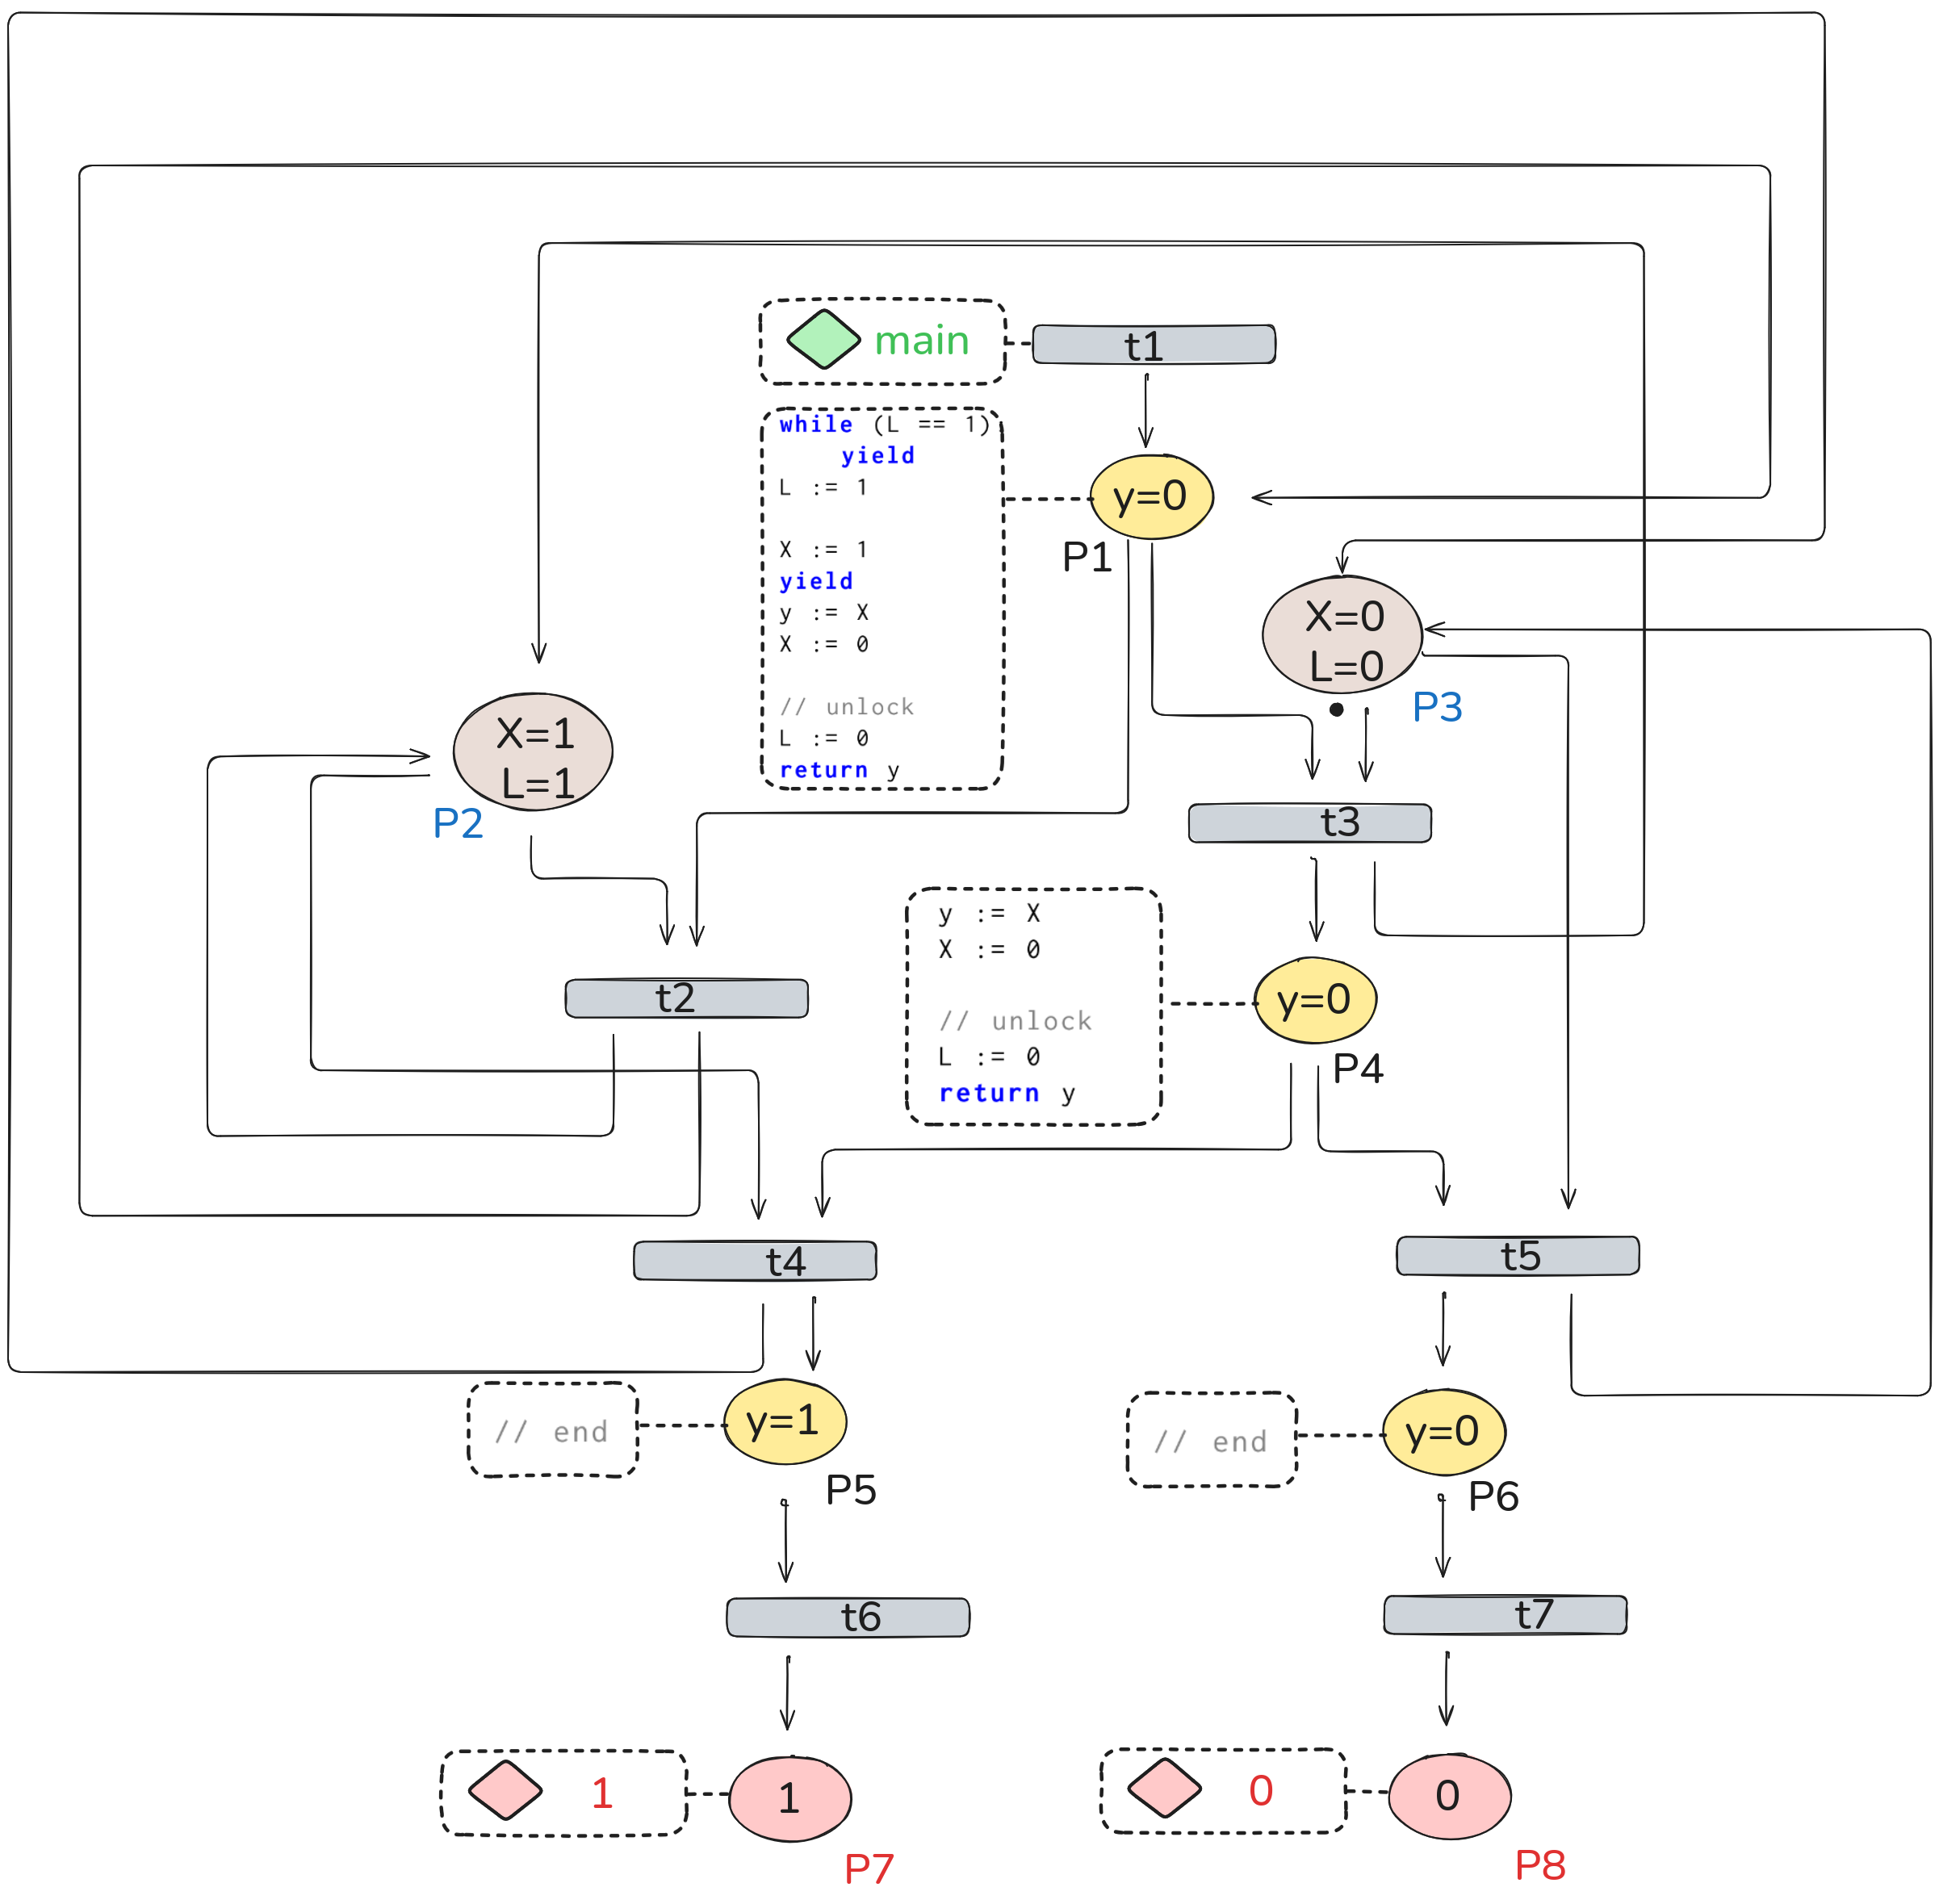
\includegraphics[width=0.8\textwidth]{plots/code_3_PN_with_annotation.png}
	\caption{Petri Net for interleaving executions of Listing~\ref{lst:MotivatingExample3Ser} program.}
	\label{fig:code3ExamplePN}
\end{figure}

\newpage